\documentclass[12pt]{article}
\usepackage{graphicx}
\usepackage{amsmath}
\usepackage{mathtools}
\usepackage{gensymb}

\newcommand{\mydet}[1]{\ensuremath{\begin{vmatrix}#1\end{vmatrix}}}
\providecommand{\brak}[1]{\ensuremath{\left(#1\right)}}
\providecommand{\norm}[1]{\left\lVert#1\right\rVert}
\providecommand{\abs}[1]{\left\vert#1\right\vert}
\newcommand{\solution}{\noindent \textbf{Solution: }}
\newcommand{\myvec}[1]{\ensuremath{\begin{pmatrix}#1\end{pmatrix}}}
\let\vec\mathbf

\begin{document}
\begin{center}
\textbf\large{CONIC SECTIONS}

\end{center}
\section*{Excercise 6.3}
Q19.Find the points on the curve $x^2+y^2-2x-3=0$ at which the tangents are parallel to the x-axis.

\solution
The equation of circle is given as
\begin{align}
	\label{eq:eq1}
	x^2 + y^2 -2x -3 = 0
\end{align}
The standard equation of circle is given by
\begin{align}
	\label{eq:eq2}
	\norm{\vec{x}}^2+2\vec{x}^\top\vec{u}+f=0
\end{align}
comparing \eqref{eq:eq1} and \eqref{eq:eq2} we get
\begin{align}
	\vec{u} &= \myvec{-1\\0}\\
	f &= -3
\end{align}
Hence, the centre and radius are given as
\begin{align}
	\vec{c} &= -\vec{u} = \myvec{1\\0}\\
	r &= \sqrt{\norm{\vec{u}}^2 - f}\\
	  &= 2
\end{align}
For a circle the point of contact of tangent are given by
\begin{align}
	\label{eq:eq3}
	\vec{q}_{ij} = \brak{\pm r\frac{\vec{n}_j}{\norm{\vec{n}_j}}-\vec{u}} \text{ i,j} = 1,2
\end{align}
Since, tangents are parallel to x-axis, the normal is given as
\begin{align}
	\vec{n} = \myvec{0\\1}
\end{align}
Substituting in \eqref{eq:eq3} we get
\begin{align}
	\vec{q}_{11} &= \brak{\pm 2\myvec{0\\1} - \myvec{-1\\0}}\\
	&= \myvec{1\\-2},\myvec{1\\2}
\end{align}
Hence, the two points of contact are
\begin{align}
	\myvec{1\\2} \text{ and } \myvec{1\\-2}
\end{align}
See Fig.\ref{fig:Fig1}.
\begin{figure}[!h]
	\begin{center} 
	    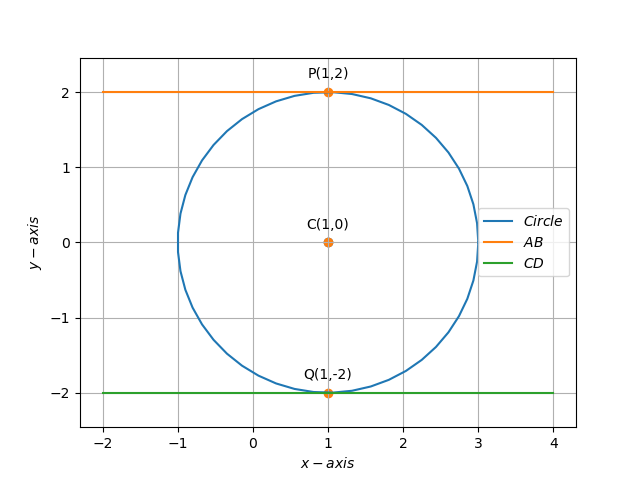
\includegraphics[width=\columnwidth]{figs/tan1}
	\end{center}
\caption{}
\label{fig:Fig1}
\end{figure}
\end{document}





















